\chapter{Computation}
Unfortunately, the explicit computations for luck may be impractical.  However, if $n$ independent samples are taken $S=(x_1, \ldots, x_n)$, then it can be estimated as: 
\begin{align*}
 \ell(x) = & \frac{1}{n} \left\{\text{\# of outcomes in S more probable than $x$}\right\}  \\
 & + \frac{1}{2n} \left\{\text{\# of outcomes in S equally probable to $x$}\right\} 
\end{align*}

It is a reasonably straightforward calculation to show that
\begin{equation}
E(\ell(x))=L(x) \,,
\end{equation}
and
\begin{equation}
E((\ell(x)-L(x))^2) \leq \frac{1}{n} L(x) \cdot (1-L(x)) \leq \frac{1}{4n}\,.
\end{equation}

\begin{example}{Multinomial.} We are aware of no computationally efficient way to exactly compute the luck for a multinomial distribution other than the explicit sum.  Suppose there is a questionnaire with 4 possible answers with category probabilities $0.1$, $0.2$, $0.3$, and $0.4$.  How lucky would it be to get $13$, $15$, $27$ and $45$ responses of each respective answer in 100 samples? 

% This example is small enough to compute the exact luck of $0.6287498$,  indicating this is a fairly typical result.

The log-probability in this case is the multinomial probability (see figure~\ref{fig:mulprobln}):
\begin{equation}
y=\text{mulprobln(x,p)}=\log \left[\left(\sum_{i=1}^{n_p} x_i \right)! \prod_{i=1}^{n_p} \frac{p_i^{x_i}}{x_i!} \right]\,.
\end{equation}

\begin{figure}
\caption{\label{fig:mulprobln}Scilab function to compute the natural log of the probability of multinomial outcomes.  $p$ is a $n_{\text{probs}} \times 1$ column vector of category probabilities, $x$ is a $n_{\text{probs}} \times n_{\text{samps}}$ matrix of outcomes, and the result {\tt lnp} is a $1 \times n_{\text{samps}}$ row vector.}
\lstset{language=Scilab}
\begin{lstlisting}
function lnp=mulprobln(x,p)
  [nprobs,nsamps]=size(x);
  pln=log(p);
  y=zeros(1,nsamps);
  for i=1:nsamps
    xi=x(:,i);
    ni=sum(xi);
    lnp(i)=gammaln(ni+1)+...
      sum(xi.*pln-gammaln(xi+1));
  end
endfunction
\end{lstlisting}
\end{figure}

Numerical estimates of luck requires samples from the given probability distribution.  Figure~\ref{fig:mulsamps} uses a built-in function in scilab to generate such a sample set.
\begin{figure}
\caption{\label{fig:mulsamps}Scilab listing to get a sample of outcomes from a multinomial distribution.  $n_{\text{samps}}$ is the number of desired samples, $n_{\text{trials}}$ is the number of trials in each sample, and $p$ is a $n_{\text{probs}} \times 1$ column vector of category probabilities.  The result $x$ is a $n_{\text{probs}} \times n_{\text{samps}}$ matrix of sample outcomes, where $\sum_{j=1}^{n_{\text{probs}}} x(j,i)=n_{\text{trials}}$.}
\lstset{language=Scilab}
\begin{lstlisting}
function x=mulsamp(nsamps,ntrials,p)
  x=grand(nsamps,"mul",ntrials,p(1:(length(p)-1)));
endfunction
\end{lstlisting}
\end{figure}

For smaller spaces, luck for a multinomial distribution can be computed explicitly.  Figure~\ref{fig:mulluck} computes this as an inefficient testing reference.
\begin{figure}
\caption{\label{fig:mulluck}Recursively compute luck of multinomial exactly using exhaustive sum.  $x$ is a $n_{\text{probs}} \times n_{\text{samps}}$ matrix of outcomes, and $p$ is a $n_{\text{probs}} \times 1$ column vector of category probabilities.  The result is a $1 \times n_{\text{samps}}$ of luck values.}
\lstset{language=Scilab}
\begin{lstlisting}
// Used by mulluck below to 
// recursively compute luck
function el=mulluckrec(nb,mb,...
              lpx,k,p,y,eps)
  [n,m]=size(lpx);
  el=zeros(n,m);
  for yk=0:nb-mb
     y(k)=yk;
     if k < length(p)-1 then
       el=el+mulluckrec(nb,mb+yk,...
         lpx,k+1,p,y,eps);
     else
       y(length(p))=nb-mb-yk;
       lpy=mulprobln(y,p);
       c=0.5*bool2s(lpy > lpx-eps)+...
           0.5*bool2s(lpy > lpx+eps);
       el = el + c .* exp(lpy);
     end
  end
endfunction

function L=mulluck(x,p,eps)
  if ~exists("eps","local") then
    eps=sqrt(%eps);
  end
  [nprobs,nsamps]=size(x);
  ntrials=sum(x,'r');
  n0=min(ntrials);
  n1=max(ntrials);
  assert_checkequal(n0,n1);
  L=mulluckrec(n0,0,mulprobln(x,p),...
      1,p,zeros(nprobs,1),eps);
endfunction
\end{lstlisting}
\end{figure}

\begin{figure}
\caption{\label{fig:numlucksetup}Given the log of the probabilities of a set of sample data, return a table used for quickly estimating luck.  {\tt problns} is a $1 \times n_{\text{nsamps}}$ row vector of logs of probabilities, and {\tt eps} is an optional parameter giving the absolute error (in log space) for considering two probabilities to be equal.  Returns {\tt setup}, a $2 \times N$ matrix giving $-\log p(x)$ and estimates for $L(x)$ for each unique probability in the sample.  This function is useful generally (not just for multinomial distributions).}
\lstset{language=Scilab}
\begin{lstlisting}
function setup=numlucksetup(problns,eps)
  if ~exists("eps","local") then
    eps=sqrt(%eps);
  end

  n=length(problns);
  problns=gsort(problns);

  for pass=1:2
    if pass == 2 then
      setup=zeros(2,count);
    end
    i=1;
    count=0;
    while i<=n
      j=i;
      while j <= n-1 & ...
          problns(i)-problns(j+1) < eps
        j=j+1;
      end
      count=count+1;
      if pass == 2 then
        setup(1,count)= ...
          -0.5*(problns(i)+problns(j));
        setup(2,count)= ...
          (i-1)/n+0.5*(j-i+1)/n;
      end
      i=j+1;
    end
  end
endfunction
\end{lstlisting}
\end{figure}

\begin{figure}
\caption{\label{fig:numluck}Estimate luck given log of probabilities and setup.  {\tt problns} is a row vector of log-probabilities, {\tt setup} is the setup from a (possibly different) sample.}
\lstset{language=Scilab}
\begin{lstlisting}
function L=numluck(problns,setup)
  L=max(0,min(1,interpln(setup,-problns)));
endfunction
\end{lstlisting}
\end{figure}

\begin{figure}
\caption{\label{fig:numluckprog}Use the above functions for estimating luck numerically ({\tt nluck}) and estimating the error in luck (numerical standard deviation).  The last lines optionally compute the exact values of luck ({\tt luck}) and standard deviations to compare with.  One run produced {\tt nluck=0.63025} and {\tt luck=0.62875} with error bound estimates {\tt nsd=0.004827}, {\tt sd=0.0048314} and {\tt z=0.3105}.}
\lstset{language=Scilab}
\begin{lstlisting}
// get sample set
nsamps=10000;
ntrials=100;
p=[0.1;0.2;0.3;0.4];
x=mulsamp(nsamps,ntrials,p);
problns=mulprobln(x,p);

// setup for luck estimates
setup=numlucksetup(problns);

// estimate luck numerically
x0=[13; 15; 27; 45];
problns0=mulprobln(x0,p);
nluck=numluck(problns0,setup);
nsd=sqrt(nluck .* (1-nluck) ./ nsamps);

// optional exact luck
luck=mulluck(x0,p);
sd=sqrt(luck .* (1-luck) ./ nsamps);

// z is approximately normally disributed
z=(nluck-luck) ./ sd;
\end{lstlisting}
\end{figure}

\begin{figure}
  \caption{Histogram of z error values for 10,000 numerical approximations of luck.  The maximum value of {\tt sd} was {\tt max(sd)=0.005}.}
  \centering
    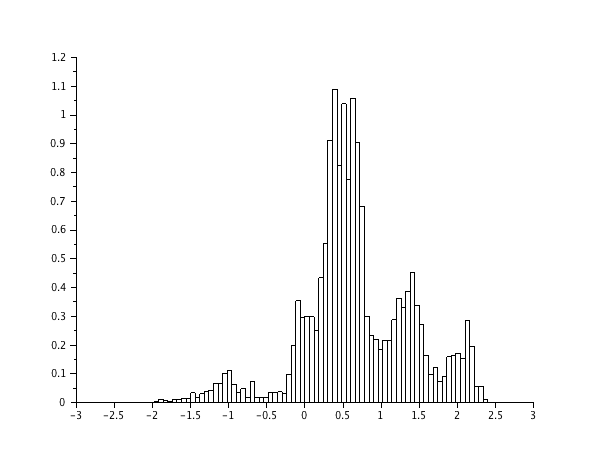
\includegraphics[width=1.00\textwidth]{img/compz.png}
\end{figure}

\end{example}
